\documentclass[12pt,a4paper]{article}

\usepackage[a4paper,text={16.5cm,25.2cm},centering]{geometry}
\usepackage{lmodern}
\usepackage{amssymb,amsmath}
\usepackage{bm}
\usepackage{graphicx}
\usepackage{microtype}
\usepackage{hyperref}
\setlength{\parindent}{0pt}
\setlength{\parskip}{1.2ex}

\hypersetup
       {   pdfauthor = { Sheehan Olver },
           pdftitle={ foo },
           colorlinks=TRUE,
           linkcolor=black,
           citecolor=blue,
           urlcolor=blue
       }




\usepackage{upquote}
\usepackage{listings}
\usepackage{xcolor}
\lstset{
    basicstyle=\ttfamily\footnotesize,
    upquote=true,
    breaklines=true,
    breakindent=0pt,
    keepspaces=true,
    showspaces=false,
    columns=fullflexible,
    showtabs=false,
    showstringspaces=false,
    escapeinside={(*@}{@*)},
    extendedchars=true,
}
\newcommand{\HLJLt}[1]{#1}
\newcommand{\HLJLw}[1]{#1}
\newcommand{\HLJLe}[1]{#1}
\newcommand{\HLJLeB}[1]{#1}
\newcommand{\HLJLo}[1]{#1}
\newcommand{\HLJLk}[1]{\textcolor[RGB]{148,91,176}{\textbf{#1}}}
\newcommand{\HLJLkc}[1]{\textcolor[RGB]{59,151,46}{\textit{#1}}}
\newcommand{\HLJLkd}[1]{\textcolor[RGB]{214,102,97}{\textit{#1}}}
\newcommand{\HLJLkn}[1]{\textcolor[RGB]{148,91,176}{\textbf{#1}}}
\newcommand{\HLJLkp}[1]{\textcolor[RGB]{148,91,176}{\textbf{#1}}}
\newcommand{\HLJLkr}[1]{\textcolor[RGB]{148,91,176}{\textbf{#1}}}
\newcommand{\HLJLkt}[1]{\textcolor[RGB]{148,91,176}{\textbf{#1}}}
\newcommand{\HLJLn}[1]{#1}
\newcommand{\HLJLna}[1]{#1}
\newcommand{\HLJLnb}[1]{#1}
\newcommand{\HLJLnbp}[1]{#1}
\newcommand{\HLJLnc}[1]{#1}
\newcommand{\HLJLncB}[1]{#1}
\newcommand{\HLJLnd}[1]{\textcolor[RGB]{214,102,97}{#1}}
\newcommand{\HLJLne}[1]{#1}
\newcommand{\HLJLneB}[1]{#1}
\newcommand{\HLJLnf}[1]{\textcolor[RGB]{66,102,213}{#1}}
\newcommand{\HLJLnfm}[1]{\textcolor[RGB]{66,102,213}{#1}}
\newcommand{\HLJLnp}[1]{#1}
\newcommand{\HLJLnl}[1]{#1}
\newcommand{\HLJLnn}[1]{#1}
\newcommand{\HLJLno}[1]{#1}
\newcommand{\HLJLnt}[1]{#1}
\newcommand{\HLJLnv}[1]{#1}
\newcommand{\HLJLnvc}[1]{#1}
\newcommand{\HLJLnvg}[1]{#1}
\newcommand{\HLJLnvi}[1]{#1}
\newcommand{\HLJLnvm}[1]{#1}
\newcommand{\HLJLl}[1]{#1}
\newcommand{\HLJLld}[1]{\textcolor[RGB]{148,91,176}{\textit{#1}}}
\newcommand{\HLJLs}[1]{\textcolor[RGB]{201,61,57}{#1}}
\newcommand{\HLJLsa}[1]{\textcolor[RGB]{201,61,57}{#1}}
\newcommand{\HLJLsb}[1]{\textcolor[RGB]{201,61,57}{#1}}
\newcommand{\HLJLsc}[1]{\textcolor[RGB]{201,61,57}{#1}}
\newcommand{\HLJLsd}[1]{\textcolor[RGB]{201,61,57}{#1}}
\newcommand{\HLJLsdB}[1]{\textcolor[RGB]{201,61,57}{#1}}
\newcommand{\HLJLsdC}[1]{\textcolor[RGB]{201,61,57}{#1}}
\newcommand{\HLJLse}[1]{\textcolor[RGB]{59,151,46}{#1}}
\newcommand{\HLJLsh}[1]{\textcolor[RGB]{201,61,57}{#1}}
\newcommand{\HLJLsi}[1]{#1}
\newcommand{\HLJLso}[1]{\textcolor[RGB]{201,61,57}{#1}}
\newcommand{\HLJLsr}[1]{\textcolor[RGB]{201,61,57}{#1}}
\newcommand{\HLJLss}[1]{\textcolor[RGB]{201,61,57}{#1}}
\newcommand{\HLJLssB}[1]{\textcolor[RGB]{201,61,57}{#1}}
\newcommand{\HLJLnB}[1]{\textcolor[RGB]{59,151,46}{#1}}
\newcommand{\HLJLnbB}[1]{\textcolor[RGB]{59,151,46}{#1}}
\newcommand{\HLJLnfB}[1]{\textcolor[RGB]{59,151,46}{#1}}
\newcommand{\HLJLnh}[1]{\textcolor[RGB]{59,151,46}{#1}}
\newcommand{\HLJLni}[1]{\textcolor[RGB]{59,151,46}{#1}}
\newcommand{\HLJLnil}[1]{\textcolor[RGB]{59,151,46}{#1}}
\newcommand{\HLJLnoB}[1]{\textcolor[RGB]{59,151,46}{#1}}
\newcommand{\HLJLoB}[1]{\textcolor[RGB]{102,102,102}{\textbf{#1}}}
\newcommand{\HLJLow}[1]{\textcolor[RGB]{102,102,102}{\textbf{#1}}}
\newcommand{\HLJLp}[1]{#1}
\newcommand{\HLJLc}[1]{\textcolor[RGB]{153,153,119}{\textit{#1}}}
\newcommand{\HLJLch}[1]{\textcolor[RGB]{153,153,119}{\textit{#1}}}
\newcommand{\HLJLcm}[1]{\textcolor[RGB]{153,153,119}{\textit{#1}}}
\newcommand{\HLJLcp}[1]{\textcolor[RGB]{153,153,119}{\textit{#1}}}
\newcommand{\HLJLcpB}[1]{\textcolor[RGB]{153,153,119}{\textit{#1}}}
\newcommand{\HLJLcs}[1]{\textcolor[RGB]{153,153,119}{\textit{#1}}}
\newcommand{\HLJLcsB}[1]{\textcolor[RGB]{153,153,119}{\textit{#1}}}
\newcommand{\HLJLg}[1]{#1}
\newcommand{\HLJLgd}[1]{#1}
\newcommand{\HLJLge}[1]{#1}
\newcommand{\HLJLgeB}[1]{#1}
\newcommand{\HLJLgh}[1]{#1}
\newcommand{\HLJLgi}[1]{#1}
\newcommand{\HLJLgo}[1]{#1}
\newcommand{\HLJLgp}[1]{#1}
\newcommand{\HLJLgs}[1]{#1}
\newcommand{\HLJLgsB}[1]{#1}
\newcommand{\HLJLgt}[1]{#1}



\def\qqand{\qquad\hbox{and}\qquad}
\def\qqfor{\qquad\hbox{for}\qquad}
\def\qqas{\qquad\hbox{as}\qquad}
\def\D{ {\rm d} }
\def\I{ {\rm i} }
\def\E{ {\rm e} }
\def\C{ {\mathbb C} }
\def\R{ {\mathbb R} }
\def\CC{ {\cal C} }
\def\HH{ {\cal H} }
\def\LL{ {\cal L} }
\def\vc#1{ {\mathbf #1} }
\def\bbC{ {\mathbb C} }

\def\qqqquad{\qquad\qquad}
\def\qqwhere{\qquad\hbox{where}\qquad}
\def\Res_#1{\underset{#1}{\rm Res}\,}
\def\sech{ {\rm sech}\, }
\def\acos{ {\rm acos}\, }
\def\atan{ {\rm atan}\, }
\def\upepsilon{\varepsilon}


\def\Xint#1{ \mathchoice
   {\XXint\displaystyle\textstyle{#1} }%
   {\XXint\textstyle\scriptstyle{#1} }%
   {\XXint\scriptstyle\scriptscriptstyle{#1} }%
   {\XXint\scriptscriptstyle\scriptscriptstyle{#1} }%
   \!\int}
\def\XXint#1#2#3{ {\setbox0=\hbox{$#1{#2#3}{\int}$}
     \vcenter{\hbox{$#2#3$}}\kern-.5\wd0} }
\def\ddashint{\Xint=}
\def\dashint{\Xint-}
% \def\dashint
\def\infdashint{\dashint_{-\infty}^\infty}




\def\addtab#1={#1\;&=}
\def\ccr{\\\addtab}
\def\ip<#1>{\left\langle{#1}\right\rangle}
\def\dx{\D x}
\def\dt{\D t}
\def\dz{\D z}

\def\norm#1{\left\| #1 \right\|}

\def\pr(#1){\left({#1}\right)}
\def\br[#1]{\left[{#1}\right]}

\def\abs#1{\left|{#1}\right|}
\def\fpr(#1){\!\pr({#1})}

\def\sopmatrix#1{ \begin{pmatrix}#1\end{pmatrix} }

\def\endash{–}
\def\mdblksquare{\blacksquare}
\def\lgblksquare{\blacksquare}
\def\scre{\E}
\def\mapengine#1,#2.{\mapfunction{#1}\ifx\void#2\else\mapengine #2.\fi }

\def\map[#1]{\mapengine #1,\void.}

\def\mapenginesep_#1#2,#3.{\mapfunction{#2}\ifx\void#3\else#1\mapengine #3.\fi }

\def\mapsep_#1[#2]{\mapenginesep_{#1}#2,\void.}


\def\vcbr[#1]{\pr(#1)}


\def\bvect[#1,#2]{
{
\def\dots{\cdots}
\def\mapfunction##1{\ | \  ##1}
	\sopmatrix{
		 \,#1\map[#2]\,
	}
}
}



\def\vect[#1]{
{\def\dots{\ldots}
	\vcbr[{#1}]
} }

\def\vectt[#1]{
{\def\dots{\ldots}
	\vect[{#1}]^{\top}
} }

\def\Vectt[#1]{
{
\def\mapfunction##1{##1 \cr} 
\def\dots{\vdots}
	\begin{pmatrix}
		\map[#1]
	\end{pmatrix}
} }

\def\addtab#1={#1\;&=}
\def\ccr{\\\addtab}

\begin{document}

\textbf{M3M6: Applied Complex Analysis}

Dr. Sheehan Olver

s.olver@imperial.ac.uk

\section{Lecture 20: Orthogonal polynomials}
We now introduce orthogonal polynomials (OPs). These are \textbf{fundamental} for computational mathematics, with applications in

\begin{itemize}
\item[1. ] Function approximation


\item[2. ] Quadrature (calculating integrals)


\item[3. ] Solving differential equations


\item[4. ] Spectral analysis of Schrödinger operators

\end{itemize}
We will investigate the properties of \emph{general} OPs, in this lecture:

\begin{itemize}
\item[1. ] Definition of orthogonal polynomials


\item[2. ] Three-term recurrence relationships


\item[3. ] Function approximation with orthogonal polynomials    


\item[4. ] Construction of orthogonal polynomials via Gram\ensuremath{\endash}Schmidt process    

\end{itemize}
\subsection{Definition of orthogonal polynomials}
Let $p_0(x),p_1(x),p_2(x),\ensuremath{\dots}$ be a sequence of polynomials such that $p_n(x)$ is exactly degree $n$, that is,

\[
p_n(x) = k_n x^n + O(x^{n-1})
\]
where $k_n \neq 0$.

Let $w(x)$ be a continuous weight function on a (possibly infinite) interval $(a,b)$: that is $w(x) \geq 0$ for all $a < x < b$.  This induces an inner product

\[
\ip<f,g> := \int_a^b f(x) g(x) w(x) \dx
\]
We say that $\{p_0, p_1,\ldots\}$ are \emph{orthogonal with respect to the weight $w$} if 

\[
\ip<p_n,p_m> = 0\qqfor n \neq m.
\]
Because $w$ is continuous, we have

\[
\norm{p_n}^2 = \ip<p_n,p_n> > 0 .
\]
Orthogonal polymomials are not unique: we can multiply each $p_n$ by a different nonzero constant $\tilde p_n(x) = c_n p_n(x)$, and  $\tilde p_n$ will be orthogonal w.r.t. $w$.  However, if we specify $k_n$, this is sufficient to uniquely define them:

\textbf{Proposition (Uniqueness of OPs I)} Given a non-zero $k_n$, there is a unique polynomial $p_n$ orthogonal w.r.t. $w$  to all lower degree polynomials.

\textbf{Proof} Suppose $r_n(x) = k_n x^n + O(x^{n-1})$ is another  OP w.r.t. $w$. We want to show $p_n - r_n$ is zero.  But this is a polynomial of degree $<n$, hence

\[
p_n(x) - r_n(x) = \sum_{k=0}^{n-1} c_k p_k(x)
\]
But we have for $k \leq n-1$

\[
\ip<p_k,p_k> c_k = \ip<p_n - r_n, p_k> = \ip<p_n,p_k> - \ip<r_n, p_k> = 0 - 0 = 0
\]
which shows all $c_k$ are zero.

\ensuremath{\blacksquare}

\textbf{Corollary (Uniqueness of OPs I)} If $q_n$ and $p_n$ are orthogonal w.r.t. $w$ to all lower degree polynomials,  then $q_n(x) = C p_n(x)$ for some constant $C$. 

\subsubsection{Monic orthogonal polynomials}
If $k_n = 1$, that is, 

\[
p_n(x) = x^n + O(x^{n-1})
\]
then we refer to the orthogonal polymomials as monic.

Monic OPs are unique as we have specified $k_n$.

\subsubsection{Orthonormal polynomials}
If  $\norm{p_n} = 1$, then we refer to the orthogonal polynomials as orthonormal w.r.t. $w$.   We will usually use $q_n$ when they are orthonormal.   Note it's not unique: we can multiply by $\pm 1$ without changing the norm.

\textbf{Remark} The classical OPs are \textbf{not} monic or orthonormal (apart from one case). Many people make the mistake of using  orthonormal polynomials for computations. But there is a good reason to use classical OPs: their properties result in rational formulae,  whereas orthonormal polynomials require square roots. This makes a performance difference.

\subsection{Function approximation with orthogonal polynomials}
A basic usage of orthogonal polynomials is for polynomial approximation.  Suppose $f(x)$ is a degree $n-1$ polynomial. Since $\{p_0(x),\ldots,p_{n-1}(x)\}$ span all degree $n-1$ polynomials, we know that

\[
f(x) = \sum_{k=0}^{n-1} f_k p_k(x)
\]
where

\[
f_k = {\ip<f, p_k> \over \ip<p_k,p_k>}
\]
Sometimes, we want to incorporate the weight into the approximation. This is typically one of two forms, depending on the application: 

\[
f(x) = w(x) \sum_{k=0}^\infty f_k p_k(x)
\]
or

\[
        f(x) = \sqrt{w(x)} \sum_{k=0}^\infty f_k p_k(x)
\]
\subsection{Jacobi operators and three-term recurences for general orthogonal polynomials}
\subsubsection{Three-term recurrence relationships}
A central theme: if you know the Jacobi operator / three-term recurrence, you know the polynomials.  This is the \textbf{best} way to evaluate expansions in orthogonal polynomials: even for cases where we have explicit formulae (e.g. Chebyshev polynomials $T_n(x) = \cos n \acos x$),  using the recurrence avoids evaluating trigonometric functions.

Every family of orthogonal polynomials has a three-term recurrence relationship:

\textbf{Theorem (three-term recurrence)} Suppose $\{p_n(x)\}$ are a family of orthogonal polynomials w.r.t. a weight $w(x)$.  Then there exists constants $a_n \neq 0$, $b_n$ and $c_n$ such that


\begin{align*}
x p_0(x) = a_0 p_0(x) + b_0 p_1(x) \\
x p_n(x) = c_n p_{n-1}(x) + a_n p_n(x) + b_n p_{n+1}(x)
\end{align*}
\textbf{Proof} The first part follows since $p_0(x)$ and $p_1(x)$ span all degree 1 polynomials.

The second part follows essentially because multiplication by $x$ is "self-adjoint", that is,

\[
\ip<x f, g> = \int_a^b x f(x) g(x) w(x) \dx = \ip<f, x g>
\]
Therefore, if $f_m$ is a degree $m < n-1$ polynomial, we have

\[
\ip<x p_n, f_m> = \ip<p_n, x f_m> = 0.
\]
In particular, if we write

\[
x p_n(x) = \sum_{k=0}^{n+1} C_k p_k(x)
\]
then

\[
C_k = {\ip< x p_n, p_k> \over \norm{p_k}^2} = 0
\]
if $k < n-1$.

\ensuremath{\blacksquare}

Monic polynomials clearly have $b_n = 1$.  Orthonormal polynomials have an even simpler form:

\textbf{Theorem (orthonormal three-term recurrence)} Suppose $\{q_n(x)\}$ are a family of orthonotms polynomials w.r.t. a weight $w(x)$.  Then there exists constants $a_n$ and $b_n$ such that


\begin{align*}
x q_0(x) = a_0 q_0(x)  + b_0 q_1(x)\\
x q_n(x) = b_{n-1} q_{n-1}(x) + a_n q_n(x) + b_{n} q_{n+1}(x)
\end{align*}
\textbf{Proof} Follows again by self-adjointness of multiplication by $x$:

\[
c_n = \ip<x q_n, q_{n-1}> = \ip<q_n, x q_{n-1}> = \ip<x q_{n-1}, q_n> = b_{n-1}
\]
\ensuremath{\blacksquare}

\textbf{Corollary (symmetric three-term recurrence implies orthonormal)} Suppose $\{p_n(x)\}$ are a family of orthogonal polynomials  w.r.t. a weight $w(x)$ such that


\begin{align*}
x p_0(x) = a_0 p_0(x)  + b_0 p_1(x)\\
x p_n(x) = b_{n-1} p_{n-1}(x) + a_n p_n(x) + b_{n} p_{n+1}(x)
\end{align*}
with $b_n \neq 0$. Suppose further that $\norm{p_0} = 1$. Then $p_n$ must be orthonormal.

\textbf{Proof} This follows from

\[
b_n = {\ip<x p_n,p_{n+1}> \over \norm{p_{n+1}}^2} = {\ip<x p_{n+1}, p_n> \over \norm{p_{n+1}}^2} = b_n   {\norm{p_n}^2 \over \norm{p_{n+1}}^2 }
\]
which implies

\[
\norm{p_{n+1}}^2 = \norm{p_n}^2 = \cdots = \norm{p_0}^2 = 1
\]
\ensuremath{\blacksquare}

\textbf{Remark} We can scale $w(x)$ by a constant without changing the orthogonality properties, hence we can make $\|p_0\| = 1$ by changing the weight.

\textbf{Remark} This is beyond the scope of this course, but satisfying a three-term recurrence like this such that coefficients  are bounded with $p_0(x) = 1$ is sufficient to show that there exists a $w(x)$ (or more accurately, a Borel measure)  such that $p_n(x)$ are orthogonal w.r.t. $w$. The relationship between the coefficients $a_n,b_n$ and the $w(x)$ is  an object of study in spectral theory, particularly when the coefficients are periodic, quasi-periodic or random.  

\subsection{Jacobi operators and multiplication by $x$}
We can rewrite the three-term recurrence as

\[
x \begin{pmatrix} p_0(x) \cr p_1(x) \cr p_2(x) \cr \vdots \end{pmatrix} = J\begin{pmatrix} p_0(x) \cr p_1(x) \cr p_2(x) \cr \vdots \end{pmatrix}
\]
where $J$ is a Jacobi operator, an infinite-dimensional tridiagonal matrix:

\[
J = \begin{pmatrix} 
a_0 & b_0 \cr
c_1 & a_1 & b_1 \cr
& c_2 & a_2 & b_2 \cr
&& c_3 & a_3 & \ddots \cr
&&&\ddots & \ddots
\end{pmatrix} 
\]
When the polynomials are monic, we have $1$ on the superdiagonal.  When we have an orthonormal basis, then $J$ is symmetric:

\[
J = \begin{pmatrix} 
a_0 & b_0 \cr
b_0 & a_1 & b_1 \cr
& b_1 & a_2 & b_2 \cr
&& b_2 & a_3 & \ddots \cr
&&&\ddots & \ddots
\end{pmatrix} 
\]
Given a polynomial expansion, $J$ tells us how to multiply by $x$ in coefficient space, that is, if

\[
f(x) = \sum_{k=0}^\infty f_k p_k(x) =   (p_0(x) ,  p_1(x) , \ldots ) \begin{pmatrix}f_0\\ f_1\\f_2\\\vdots\end{pmatrix}
\]
then (provided the relevant sums converge absolutely and uniformly)

\[
x f(x) = x (p_0(x) ,  p_1(x) , \ldots ) \begin{pmatrix}f_0\\ f_1\\f_2\\\vdots\end{pmatrix} =
    \left(J \begin{pmatrix} p_0(x) \cr p_1(x) \cr p_2(x) \cr \vdots \end{pmatrix}\right)^\top  \begin{pmatrix}f_0\\ f_1\\f_2\\\vdots\end{pmatrix} = (p_0(x) ,  p_1(x) , \ldots ) X \begin{pmatrix}f_0\\ f_1\\f_2\\\vdots\end{pmatrix}
\]
where $X := J^\top$. 

\subsubsection{Evaluating polynomials}
We can use the three-term recurrence to construct the polynomials.  I think it's nicest to express this in terms of linear algebra.  Suppose we are given $p_0(x) = k_0$ (where $k_0 = 1$ is pretty much always the case in practice). This can be written in matrix form as

\[
(1,0,0,0,0,\ldots) \begin{pmatrix} p_0(x) \cr p_1(x) \cr p_2(x) \cr \vdots \end{pmatrix} = k_0
\]
We can combine this with the Jacobi operator to get

\[
\underbrace{\begin{pmatrix}
1 \\
a_0-x & b_0 \\
c_1 & a_1-x & b_1 \\
& c_2 & a_2-x & b_2 \cr
&& c_3 & a_3-x & b_3 \cr
&&&\ddots & \ddots & \ddots
\end{pmatrix}}_{L_x} \begin{pmatrix} p_0(x) \cr p_1(x) \cr p_2(x) \cr \vdots \end{pmatrix} = \begin{pmatrix} k_0\cr 0 \cr 0 \cr \vdots \end{pmatrix}
\]
For $x$ fixed, this is a lower triangular system, that is, the polynomials equal 

\[
k_0 L_x^{-1} \vc e_0
\]
This  can be solved  via forward recurrence:


\begin{align*}
    p_0(x) &= k_0 \\
    p_1(x) &= {(x-a_0) p_0(x) \over b_0}\\
    p_2(x) &= {(x-a_1) p_0(x) - c_1 p_0(x) \over b_1}\\    
    p_3(x) &= {(x-a_2) p_1(x) - c_2 p_1(x) \over b_2}\\ 
    &\vdots
\end{align*}
We can use this to evaluate functions as well: 

\[
f(x) = (p_0(x),p_1(x),\ldots) \begin{pmatrix}f_0 \\ f_1\\ \vdots \end{pmatrix} = 
k_0 \vc e_0^\top L_x^{-\top}  \begin{pmatrix}f_0 \\ f_1\\ \vdots \end{pmatrix}
\]
when $f$ is a degree $n-1$ polynomial, this becomes a problem of inverting an upper triangular matrix,  that is, we want to solve the $n \times n$ system

\[
\underbrace{\begin{pmatrix}
1 & a_0-x & c_1 \\
& b_0 & a_1-x & c_2  \\
& & b_1 & a_2-x & \ddots  \\
& &     & b_2 & \ddots & c_{n-2} \\
&&&&\ddots & a_{n-2}-x \\
&&&&& b_{n-2}
\end{pmatrix}}_{L_x^\top} \begin{pmatrix} \gamma_0 \\\vdots\\ \gamma_{n-1} \end{pmatrix}
\]
so that $f(x) = \gamma_0$. We we can solve this  via back-substitution:


\begin{align*}
\gamma_{n-1} &= {f_{n-1} \over b_{n-2}} \\
\gamma_{n-2} &= {f_{n-2} - (a_{n-2}-x) \gamma_{n-1} \over b_{n-3}} \\
\gamma_{n-3} &= {f_{n-3} - (a_{n-3}-x) \gamma_{n-2} - c_{n-2} \gamma_{n-1} \over b_{n-4}} \\
& \vdots \\
\gamma_1 &= {f_1 - (a_1-x) \gamma_2 - c_2 \gamma_3 \over b_0} \\
\gamma_0 &= f_0 - (a_0-x) \gamma_1 - c_1 \gamma_2
\end{align*}
We give examples of these algorithms applied to Chebyshev polynomials in the next lecture.

\subsection{Gram\ensuremath{\endash}Schmidt algorithm}
In general we don't have nice formulae. But we can always construct them via Gram\ensuremath{\endash}Schmidt:

\textbf{Proposition (Gram\ensuremath{\endash}Schmidt)} Define


\begin{align*}
p_0(x) = 1 \\
q_0(x) = {1 \over \norm{p_0}}\\
p_{n+1}(x) = x q_n(x) - \sum_{k=0}^n \ip<x q_n, q_k> q_k(x)\\
q_{n+1}(x) = {p_{n+1}(x) \over \norm{p_n}}
\end{align*}
Then $q_0(x), q_1(x), \ldots$ are orthonormal w.r.t. $w$.

\textbf{Proof} By linearity we have

\[
\ip<p_{n+1}, q_j> = \ip<x q_n - \sum_{k=0}^n {\ip<x q_n, q_k>} q_k, q_j> = \ip<x q_n, q_j> - \ip<x q_n, q_j> \ip<q_j,q_j> = 0
\]
Thus $p_{n+1}$ is orthogonal to all lower degree polynomials. So is $q_{n+1}$, since it is a constant multiple of $p_{n+1}$.

\ensuremath{\blacksquare}

Let's make our own family:


\begin{lstlisting}
(*@\HLJLk{using}@*) (*@\HLJLn{ApproxFun}@*)(*@\HLJLp{,}@*) (*@\HLJLn{Plots}@*)
(*@\HLJLn{x}@*) (*@\HLJLoB{=}@*) (*@\HLJLnf{Fun}@*)(*@\HLJLp{()}@*)
(*@\HLJLn{w}@*) (*@\HLJLoB{=}@*) (*@\HLJLnf{exp}@*)(*@\HLJLp{(}@*)(*@\HLJLn{x}@*)(*@\HLJLp{)}@*)
(*@\HLJLn{ip}@*) (*@\HLJLoB{=}@*) (*@\HLJLp{(}@*)(*@\HLJLn{f}@*)(*@\HLJLp{,}@*)(*@\HLJLn{g}@*)(*@\HLJLp{)}@*) (*@\HLJLoB{->}@*) (*@\HLJLnf{sum}@*)(*@\HLJLp{(}@*)(*@\HLJLn{f}@*)(*@\HLJLoB{*}@*)(*@\HLJLn{g}@*)(*@\HLJLoB{*}@*)(*@\HLJLn{w}@*)(*@\HLJLp{)}@*)
(*@\HLJLn{nrm}@*) (*@\HLJLoB{=}@*) (*@\HLJLn{f}@*)    (*@\HLJLoB{->}@*) (*@\HLJLnf{sqrt}@*)(*@\HLJLp{(}@*)(*@\HLJLnf{ip}@*)(*@\HLJLp{(}@*)(*@\HLJLn{f}@*)(*@\HLJLp{,}@*)(*@\HLJLn{f}@*)(*@\HLJLp{))}@*)
(*@\HLJLn{n}@*) (*@\HLJLoB{=}@*) (*@\HLJLni{10}@*)
(*@\HLJLn{q}@*) (*@\HLJLoB{=}@*) (*@\HLJLnf{Array}@*)(*@\HLJLp{{\{}}@*)(*@\HLJLn{Fun}@*)(*@\HLJLp{{\}}(}@*)(*@\HLJLn{undef}@*)(*@\HLJLp{,}@*)(*@\HLJLn{n}@*)(*@\HLJLp{)}@*)
(*@\HLJLn{p}@*) (*@\HLJLoB{=}@*) (*@\HLJLnf{Array}@*)(*@\HLJLp{{\{}}@*)(*@\HLJLn{Fun}@*)(*@\HLJLp{{\}}(}@*)(*@\HLJLn{undef}@*)(*@\HLJLp{,}@*)(*@\HLJLn{n}@*)(*@\HLJLp{)}@*)
(*@\HLJLn{p}@*)(*@\HLJLp{[}@*)(*@\HLJLni{1}@*)(*@\HLJLp{]}@*) (*@\HLJLoB{=}@*) (*@\HLJLnf{Fun}@*)(*@\HLJLp{(}@*)(*@\HLJLni{1}@*)(*@\HLJLp{,}@*) (*@\HLJLoB{-}@*)(*@\HLJLni{1}@*) (*@\HLJLoB{..}@*) (*@\HLJLni{1}@*) (*@\HLJLp{)}@*)
(*@\HLJLn{q}@*)(*@\HLJLp{[}@*)(*@\HLJLni{1}@*)(*@\HLJLp{]}@*) (*@\HLJLoB{=}@*) (*@\HLJLn{p}@*)(*@\HLJLp{[}@*)(*@\HLJLni{1}@*)(*@\HLJLp{]}@*)(*@\HLJLoB{/}@*)(*@\HLJLnf{nrm}@*)(*@\HLJLp{(}@*)(*@\HLJLn{p}@*)(*@\HLJLp{[}@*)(*@\HLJLni{1}@*)(*@\HLJLp{])}@*)

(*@\HLJLk{for}@*) (*@\HLJLn{k}@*)(*@\HLJLoB{=}@*)(*@\HLJLni{1}@*)(*@\HLJLoB{:}@*)(*@\HLJLn{n}@*)(*@\HLJLoB{-}@*)(*@\HLJLni{1}@*)
    (*@\HLJLn{p}@*)(*@\HLJLp{[}@*)(*@\HLJLn{k}@*)(*@\HLJLoB{+}@*)(*@\HLJLni{1}@*)(*@\HLJLp{]}@*) (*@\HLJLoB{=}@*) (*@\HLJLn{x}@*)(*@\HLJLoB{*}@*)(*@\HLJLn{q}@*)(*@\HLJLp{[}@*)(*@\HLJLn{k}@*)(*@\HLJLp{]}@*) 
    (*@\HLJLk{for}@*) (*@\HLJLn{j}@*)(*@\HLJLoB{=}@*)(*@\HLJLni{1}@*)(*@\HLJLoB{:}@*)(*@\HLJLn{k}@*)
        (*@\HLJLn{p}@*)(*@\HLJLp{[}@*)(*@\HLJLn{k}@*)(*@\HLJLoB{+}@*)(*@\HLJLni{1}@*)(*@\HLJLp{]}@*) (*@\HLJLoB{-=}@*) (*@\HLJLnf{ip}@*)(*@\HLJLp{(}@*)(*@\HLJLn{p}@*)(*@\HLJLp{[}@*)(*@\HLJLn{k}@*)(*@\HLJLoB{+}@*)(*@\HLJLni{1}@*)(*@\HLJLp{],}@*)(*@\HLJLn{q}@*)(*@\HLJLp{[}@*)(*@\HLJLn{j}@*)(*@\HLJLp{])}@*)(*@\HLJLoB{*}@*)(*@\HLJLn{q}@*)(*@\HLJLp{[}@*)(*@\HLJLn{j}@*)(*@\HLJLp{]}@*)
    (*@\HLJLk{end}@*)
    (*@\HLJLn{q}@*)(*@\HLJLp{[}@*)(*@\HLJLn{k}@*)(*@\HLJLoB{+}@*)(*@\HLJLni{1}@*)(*@\HLJLp{]}@*) (*@\HLJLoB{=}@*) (*@\HLJLn{p}@*)(*@\HLJLp{[}@*)(*@\HLJLn{k}@*)(*@\HLJLoB{+}@*)(*@\HLJLni{1}@*)(*@\HLJLp{]}@*)(*@\HLJLoB{/}@*)(*@\HLJLnf{nrm}@*)(*@\HLJLp{(}@*)(*@\HLJLn{p}@*)(*@\HLJLp{[}@*)(*@\HLJLn{k}@*)(*@\HLJLoB{+}@*)(*@\HLJLni{1}@*)(*@\HLJLp{])}@*)
(*@\HLJLk{end}@*)

(*@\HLJLnf{sum}@*)(*@\HLJLp{(}@*)(*@\HLJLn{q}@*)(*@\HLJLp{[}@*)(*@\HLJLni{2}@*)(*@\HLJLp{]}@*)(*@\HLJLoB{*}@*)(*@\HLJLn{q}@*)(*@\HLJLp{[}@*)(*@\HLJLni{4}@*)(*@\HLJLp{]}@*)(*@\HLJLoB{*}@*)(*@\HLJLn{w}@*)(*@\HLJLp{)}@*)

(*@\HLJLn{p}@*) (*@\HLJLoB{=}@*) (*@\HLJLnf{plot}@*)(*@\HLJLp{(;}@*) (*@\HLJLn{legend}@*)(*@\HLJLoB{=}@*)(*@\HLJLkc{false}@*)(*@\HLJLp{)}@*)
(*@\HLJLk{for}@*) (*@\HLJLn{k}@*)(*@\HLJLoB{=}@*)(*@\HLJLni{1}@*)(*@\HLJLoB{:}@*)(*@\HLJLni{10}@*)
    (*@\HLJLnf{plot!}@*)(*@\HLJLp{(}@*)(*@\HLJLn{q}@*)(*@\HLJLp{[}@*)(*@\HLJLn{k}@*)(*@\HLJLp{])}@*)
(*@\HLJLk{end}@*)
(*@\HLJLn{p}@*)
\end{lstlisting}

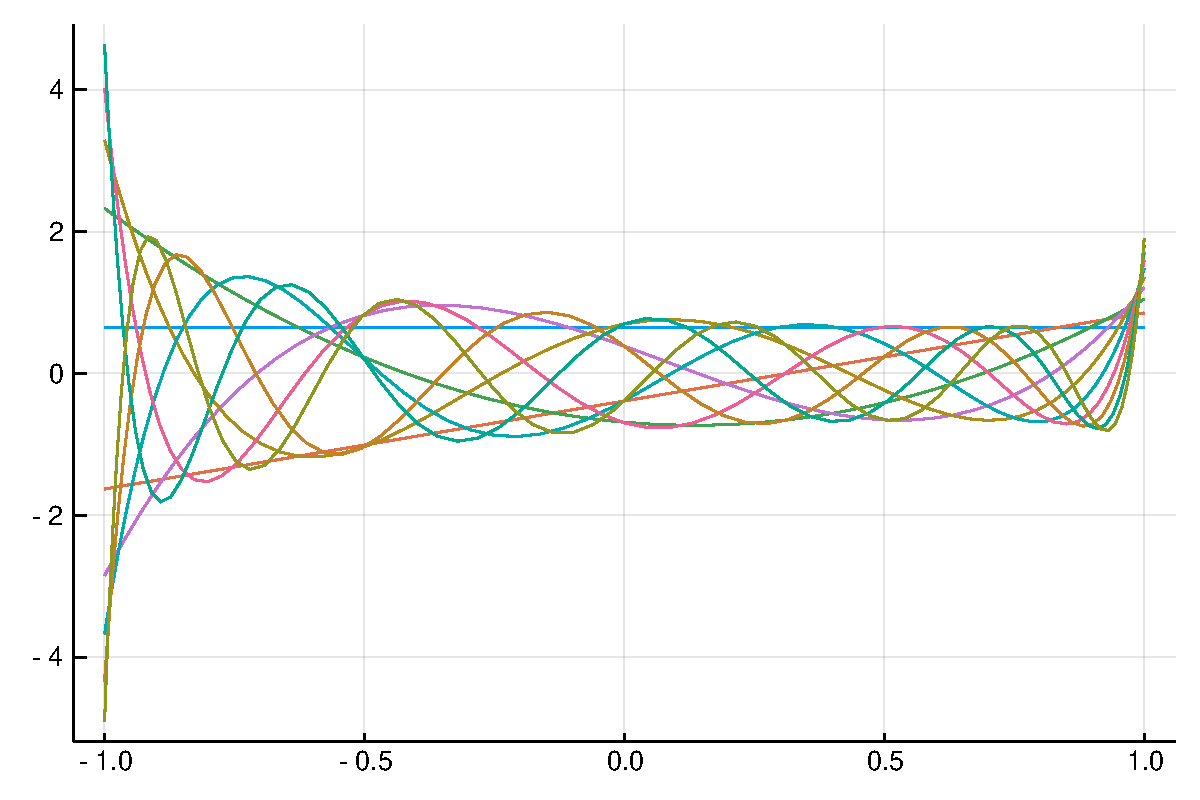
\includegraphics[width=\linewidth]{figures/Lecture20_1_1.pdf}

The three-term recurrence means we can simplify Gram\ensuremath{\endash}Schmidt, and calculate the recurrence coefficients at the same time:

\textbf{Proposition (Gram\ensuremath{\endash}Schmidt)} Define


\begin{align*}
p_0(x) &= 1 \\
q_0(x) &= {1 \over \norm{p_0}}\\
a_n &= \ip<x q_n, q_n> \\
b_{n-1} &= \ip<x q_n, q_{n-1}>\\
p_{n+1}(x) &= x q_n(x) -  a_n q_n(x) -  b_{n-1} q_{n-1}(x)\\
q_{n+1}(x) &= {p_{n+1}(x) \over \norm{p_n}}
\end{align*}
Then $q_0(x), q_1(x), \ldots$ are orthonormal w.r.t. $w$.

\textbf{Remark} This can be made a bit more efficient by using $\norm{p_n}$ to calculate $b_n$.


\begin{lstlisting}
(*@\HLJLn{x}@*) (*@\HLJLoB{=}@*) (*@\HLJLnf{Fun}@*)(*@\HLJLp{()}@*)
(*@\HLJLn{w}@*) (*@\HLJLoB{=}@*) (*@\HLJLnf{exp}@*)(*@\HLJLp{(}@*)(*@\HLJLn{x}@*)(*@\HLJLp{)}@*)
(*@\HLJLn{ip}@*) (*@\HLJLoB{=}@*) (*@\HLJLp{(}@*)(*@\HLJLn{f}@*)(*@\HLJLp{,}@*)(*@\HLJLn{g}@*)(*@\HLJLp{)}@*) (*@\HLJLoB{->}@*) (*@\HLJLnf{sum}@*)(*@\HLJLp{(}@*)(*@\HLJLn{f}@*)(*@\HLJLoB{*}@*)(*@\HLJLn{g}@*)(*@\HLJLoB{*}@*)(*@\HLJLn{w}@*)(*@\HLJLp{)}@*)
(*@\HLJLn{nrm}@*) (*@\HLJLoB{=}@*) (*@\HLJLn{f}@*)    (*@\HLJLoB{->}@*) (*@\HLJLnf{sqrt}@*)(*@\HLJLp{(}@*)(*@\HLJLnf{ip}@*)(*@\HLJLp{(}@*)(*@\HLJLn{f}@*)(*@\HLJLp{,}@*)(*@\HLJLn{f}@*)(*@\HLJLp{))}@*)
(*@\HLJLn{n}@*) (*@\HLJLoB{=}@*) (*@\HLJLni{10}@*)
(*@\HLJLn{q}@*) (*@\HLJLoB{=}@*) (*@\HLJLnf{Array}@*)(*@\HLJLp{{\{}}@*)(*@\HLJLn{Fun}@*)(*@\HLJLp{{\}}(}@*)(*@\HLJLn{undef}@*)(*@\HLJLp{,}@*) (*@\HLJLn{n}@*)(*@\HLJLp{)}@*)
(*@\HLJLn{p}@*) (*@\HLJLoB{=}@*) (*@\HLJLnf{Array}@*)(*@\HLJLp{{\{}}@*)(*@\HLJLn{Fun}@*)(*@\HLJLp{{\}}(}@*)(*@\HLJLn{undef}@*)(*@\HLJLp{,}@*) (*@\HLJLn{n}@*)(*@\HLJLp{)}@*)
(*@\HLJLn{a}@*) (*@\HLJLoB{=}@*) (*@\HLJLnf{zeros}@*)(*@\HLJLp{(}@*)(*@\HLJLn{n}@*)(*@\HLJLp{)}@*)
(*@\HLJLn{b}@*) (*@\HLJLoB{=}@*) (*@\HLJLnf{zeros}@*)(*@\HLJLp{(}@*)(*@\HLJLn{n}@*)(*@\HLJLp{)}@*)
(*@\HLJLn{p}@*)(*@\HLJLp{[}@*)(*@\HLJLni{1}@*)(*@\HLJLp{]}@*) (*@\HLJLoB{=}@*) (*@\HLJLnf{Fun}@*)(*@\HLJLp{(}@*)(*@\HLJLni{1}@*)(*@\HLJLp{,}@*) (*@\HLJLoB{-}@*)(*@\HLJLni{1}@*) (*@\HLJLoB{..}@*) (*@\HLJLni{1}@*) (*@\HLJLp{)}@*)
(*@\HLJLn{q}@*)(*@\HLJLp{[}@*)(*@\HLJLni{1}@*)(*@\HLJLp{]}@*) (*@\HLJLoB{=}@*) (*@\HLJLn{p}@*)(*@\HLJLp{[}@*)(*@\HLJLni{1}@*)(*@\HLJLp{]}@*)(*@\HLJLoB{/}@*)(*@\HLJLnf{nrm}@*)(*@\HLJLp{(}@*)(*@\HLJLn{p}@*)(*@\HLJLp{[}@*)(*@\HLJLni{1}@*)(*@\HLJLp{])}@*)

(*@\HLJLn{p}@*)(*@\HLJLp{[}@*)(*@\HLJLni{2}@*)(*@\HLJLp{]}@*) (*@\HLJLoB{=}@*) (*@\HLJLn{x}@*)(*@\HLJLoB{*}@*)(*@\HLJLn{q}@*)(*@\HLJLp{[}@*)(*@\HLJLni{1}@*)(*@\HLJLp{]}@*)
(*@\HLJLn{a}@*)(*@\HLJLp{[}@*)(*@\HLJLni{1}@*)(*@\HLJLp{]}@*) (*@\HLJLoB{=}@*) (*@\HLJLnf{ip}@*)(*@\HLJLp{(}@*)(*@\HLJLn{p}@*)(*@\HLJLp{[}@*)(*@\HLJLni{2}@*)(*@\HLJLp{],}@*)(*@\HLJLn{q}@*)(*@\HLJLp{[}@*)(*@\HLJLni{1}@*)(*@\HLJLp{])}@*)
(*@\HLJLn{p}@*)(*@\HLJLp{[}@*)(*@\HLJLni{2}@*)(*@\HLJLp{]}@*) (*@\HLJLoB{-=}@*) (*@\HLJLn{a}@*)(*@\HLJLp{[}@*)(*@\HLJLni{1}@*)(*@\HLJLp{]}@*)(*@\HLJLoB{*}@*)(*@\HLJLn{q}@*)(*@\HLJLp{[}@*)(*@\HLJLni{1}@*)(*@\HLJLp{]}@*)
(*@\HLJLn{q}@*)(*@\HLJLp{[}@*)(*@\HLJLni{2}@*)(*@\HLJLp{]}@*) (*@\HLJLoB{=}@*) (*@\HLJLn{p}@*)(*@\HLJLp{[}@*)(*@\HLJLni{2}@*)(*@\HLJLp{]}@*)(*@\HLJLoB{/}@*)(*@\HLJLnf{nrm}@*)(*@\HLJLp{(}@*)(*@\HLJLn{p}@*)(*@\HLJLp{[}@*)(*@\HLJLni{2}@*)(*@\HLJLp{])}@*)

(*@\HLJLk{for}@*) (*@\HLJLn{k}@*)(*@\HLJLoB{=}@*)(*@\HLJLni{2}@*)(*@\HLJLoB{:}@*)(*@\HLJLn{n}@*)(*@\HLJLoB{-}@*)(*@\HLJLni{1}@*)
    (*@\HLJLn{p}@*)(*@\HLJLp{[}@*)(*@\HLJLn{k}@*)(*@\HLJLoB{+}@*)(*@\HLJLni{1}@*)(*@\HLJLp{]}@*) (*@\HLJLoB{=}@*) (*@\HLJLn{x}@*)(*@\HLJLoB{*}@*)(*@\HLJLn{q}@*)(*@\HLJLp{[}@*)(*@\HLJLn{k}@*)(*@\HLJLp{]}@*) 
    (*@\HLJLn{b}@*)(*@\HLJLp{[}@*)(*@\HLJLn{k}@*)(*@\HLJLoB{-}@*)(*@\HLJLni{1}@*)(*@\HLJLp{]}@*) (*@\HLJLoB{=}@*)(*@\HLJLnf{ip}@*)(*@\HLJLp{(}@*)(*@\HLJLn{p}@*)(*@\HLJLp{[}@*)(*@\HLJLn{k}@*)(*@\HLJLoB{+}@*)(*@\HLJLni{1}@*)(*@\HLJLp{],}@*)(*@\HLJLn{q}@*)(*@\HLJLp{[}@*)(*@\HLJLn{k}@*)(*@\HLJLoB{-}@*)(*@\HLJLni{1}@*)(*@\HLJLp{])}@*)
    (*@\HLJLn{a}@*)(*@\HLJLp{[}@*)(*@\HLJLn{k}@*)(*@\HLJLp{]}@*) (*@\HLJLoB{=}@*) (*@\HLJLnf{ip}@*)(*@\HLJLp{(}@*)(*@\HLJLn{p}@*)(*@\HLJLp{[}@*)(*@\HLJLn{k}@*)(*@\HLJLoB{+}@*)(*@\HLJLni{1}@*)(*@\HLJLp{],}@*)(*@\HLJLn{q}@*)(*@\HLJLp{[}@*)(*@\HLJLn{k}@*)(*@\HLJLp{])}@*)
    (*@\HLJLn{p}@*)(*@\HLJLp{[}@*)(*@\HLJLn{k}@*)(*@\HLJLoB{+}@*)(*@\HLJLni{1}@*)(*@\HLJLp{]}@*) (*@\HLJLoB{=}@*) (*@\HLJLn{p}@*)(*@\HLJLp{[}@*)(*@\HLJLn{k}@*)(*@\HLJLoB{+}@*)(*@\HLJLni{1}@*)(*@\HLJLp{]}@*) (*@\HLJLoB{-}@*) (*@\HLJLn{a}@*)(*@\HLJLp{[}@*)(*@\HLJLn{k}@*)(*@\HLJLp{]}@*)(*@\HLJLn{q}@*)(*@\HLJLp{[}@*)(*@\HLJLn{k}@*)(*@\HLJLp{]}@*) (*@\HLJLoB{-}@*) (*@\HLJLn{b}@*)(*@\HLJLp{[}@*)(*@\HLJLn{k}@*)(*@\HLJLoB{-}@*)(*@\HLJLni{1}@*)(*@\HLJLp{]}@*)(*@\HLJLn{q}@*)(*@\HLJLp{[}@*)(*@\HLJLn{k}@*)(*@\HLJLoB{-}@*)(*@\HLJLni{1}@*)(*@\HLJLp{]}@*)
    (*@\HLJLn{q}@*)(*@\HLJLp{[}@*)(*@\HLJLn{k}@*)(*@\HLJLoB{+}@*)(*@\HLJLni{1}@*)(*@\HLJLp{]}@*) (*@\HLJLoB{=}@*) (*@\HLJLn{p}@*)(*@\HLJLp{[}@*)(*@\HLJLn{k}@*)(*@\HLJLoB{+}@*)(*@\HLJLni{1}@*)(*@\HLJLp{]}@*)(*@\HLJLoB{/}@*)(*@\HLJLnf{nrm}@*)(*@\HLJLp{(}@*)(*@\HLJLn{p}@*)(*@\HLJLp{[}@*)(*@\HLJLn{k}@*)(*@\HLJLoB{+}@*)(*@\HLJLni{1}@*)(*@\HLJLp{])}@*)
(*@\HLJLk{end}@*)

(*@\HLJLnf{ip}@*)(*@\HLJLp{(}@*)(*@\HLJLn{q}@*)(*@\HLJLp{[}@*)(*@\HLJLni{5}@*)(*@\HLJLp{],}@*)(*@\HLJLn{q}@*)(*@\HLJLp{[}@*)(*@\HLJLni{2}@*)(*@\HLJLp{])}@*) (*@\HLJLcs{{\#}}@*) (*@\HLJLcs{shows}@*) (*@\HLJLcs{orthogonality}@*) (*@\HLJLcs{(to}@*) (*@\HLJLcs{numerical}@*) (*@\HLJLcs{accuracy)}@*)
\end{lstlisting}

\begin{lstlisting}
5.828670879282072e-16
\end{lstlisting}


Here we see a plot of the first 10 polynomials:


\begin{lstlisting}
(*@\HLJLn{p}@*) (*@\HLJLoB{=}@*) (*@\HLJLnf{plot}@*)(*@\HLJLp{(;}@*) (*@\HLJLn{legend}@*)(*@\HLJLoB{=}@*)(*@\HLJLkc{false}@*)(*@\HLJLp{)}@*)
(*@\HLJLk{for}@*) (*@\HLJLn{k}@*)(*@\HLJLoB{=}@*)(*@\HLJLni{1}@*)(*@\HLJLoB{:}@*)(*@\HLJLni{10}@*)
    (*@\HLJLnf{plot!}@*)(*@\HLJLp{(}@*)(*@\HLJLn{q}@*)(*@\HLJLp{[}@*)(*@\HLJLn{k}@*)(*@\HLJLp{])}@*)
(*@\HLJLk{end}@*)
(*@\HLJLn{p}@*)
\end{lstlisting}

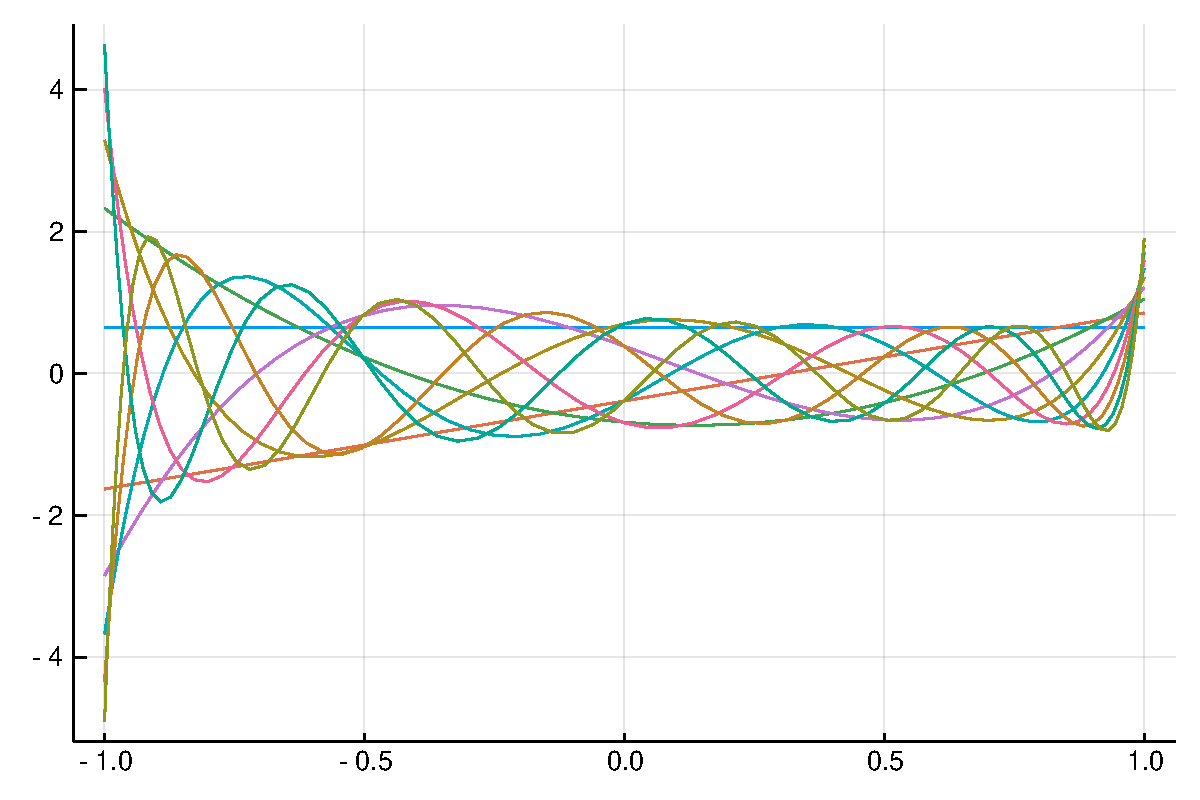
\includegraphics[width=\linewidth]{figures/Lecture20_3_1.pdf}


\end{document}
